% ------------------------------------------------------------------------------------------------
% TeX template for university, written by Leandro Ebner 2023.
% v0.1.0-beta, licensed under the GNU GPLv3, see "LICENSE" and <https://www.gnu.org/licenses/>
% ------------------------------------------------------------------------------------------------

\documentclass{scrartcl}                    % use KOMA-Script class "article"
\usepackage{rwudefs}                        % use RWU template
\usepackage{biblatex}                       % required to use external bibliography file, unfortunately IEEE is only available when comp. in overleaf
\addbibresource{bibliography.bib}           % main directory for bibliography
\usepackage[automark]{scrlayer-scrpage}     % use custom header and footer
\clearpairofpagestyles                      % clear default values of header and footer
\setlength{\headheight}{53pt}               % adjust header to fit in RWU logo
\setlength{\footheight}{41pt}               % adjusts footer to fit GPL logo
\ohead[\rwulogo]{\headmark}                 % set custom header
\ofoot[\pagemark]{\pagemark}                % set custom footer
\ifoot[]{© Leandro Ebner 2023}              % copyright emblem
\usepackage{graphicx}                       % required for inserting images
\graphicspath{{graphicx/}}                  % main directory for images
\usepackage{svg}                            % ability to use svg 
\usepackage{wrapfig}                        % package to embedd smaller pictures more appeiling
\usepackage{layout}                         % for debugging typeset only
\usepackage{hyperref}                       % allows for links in references and labels
\usepackage{listings}                       % required to embed code

\lstset{                                    % settings for package "listings"
    language=C++,
    numbers=left, 
    keywordstyle=\color{magenta}\bfseries}
\hypersetup{                                % settings for package "hyperref"
    colorlinks=true,
    linkcolor=blue,
    citecolor=blue,      
    urlcolor=cyan,
    pdftitle={Leandro Ebner Task 4},
    pdfpagemode=FullScreen}
    
\ifoot[
\includegraphics{graphicx/gplv3-or-later.png}]{}
\cfoot[Copyright 2023 © Leandro Ebner \\ Licensed under the GNU GPLv3, \\ see \href{https://www.gnu.org/licenses/gpl.html}{https://www.gnu.org/licenses/gpl.html}]{}   


% main code:

\begin{document}

\title{Microcontroller Task 4}
\author{Ebner, Leandro et al.\thanks{Caleb Patrick DSouza, Matr. Nr.: 28840332} \\ Matr. Nr.: 14740284}
\date{\today}
\maketitle

\begin{abstract}
Grundpraktikum 3: \\ Control of an RC servo by an IR remote control and an optical sensor. \\
Written with the help of KOMA-Script in \LaTeXe{}.
\end{abstract}

\tableofcontents
\newpage

\section{Introduction}

The aim of the “Task 4. Control of an RC servo by an IR remote control and an optical sensor” is making the participants able to do the following task below:
\begin{enumerate}
    \item Create the hardware setup.
    \item Implement the infrared receiver function.
    \item Implement the servo motor control function.
    \item Implement the reflective sensor function.
\end{enumerate}

\section{Basic theory}
    \subsection{Arduino Nano}

    The \emph{Arduino Nano} is a development board that is based on the \emph{ATmega328P} microcontroller. It is part of the Arduino family \cite{arduino} of open source hardware and software products, which are designed to facilitate electronic prototyping. The Nano model, in particular, is known for it's small size, affordability, and a wide range of applications. Thus it can be used easily with the \emph{Arduino IDE} which is an ideal choice for both beginners and experienced users. The microcontroller is equipped with 32kB of flash memory, 2kB of SRAM, and 1kB of EEPROM. It can control other devices and components with the help of 14 digital input/output pins and 8 analog pins. Powering and uploading the code can be done by utilising the modern USB-C connector of the Arduino Nano. A more detailed figure of the pinout is given at figure \ref{pinout}.

    \begin{figure}[h]
        \centering
        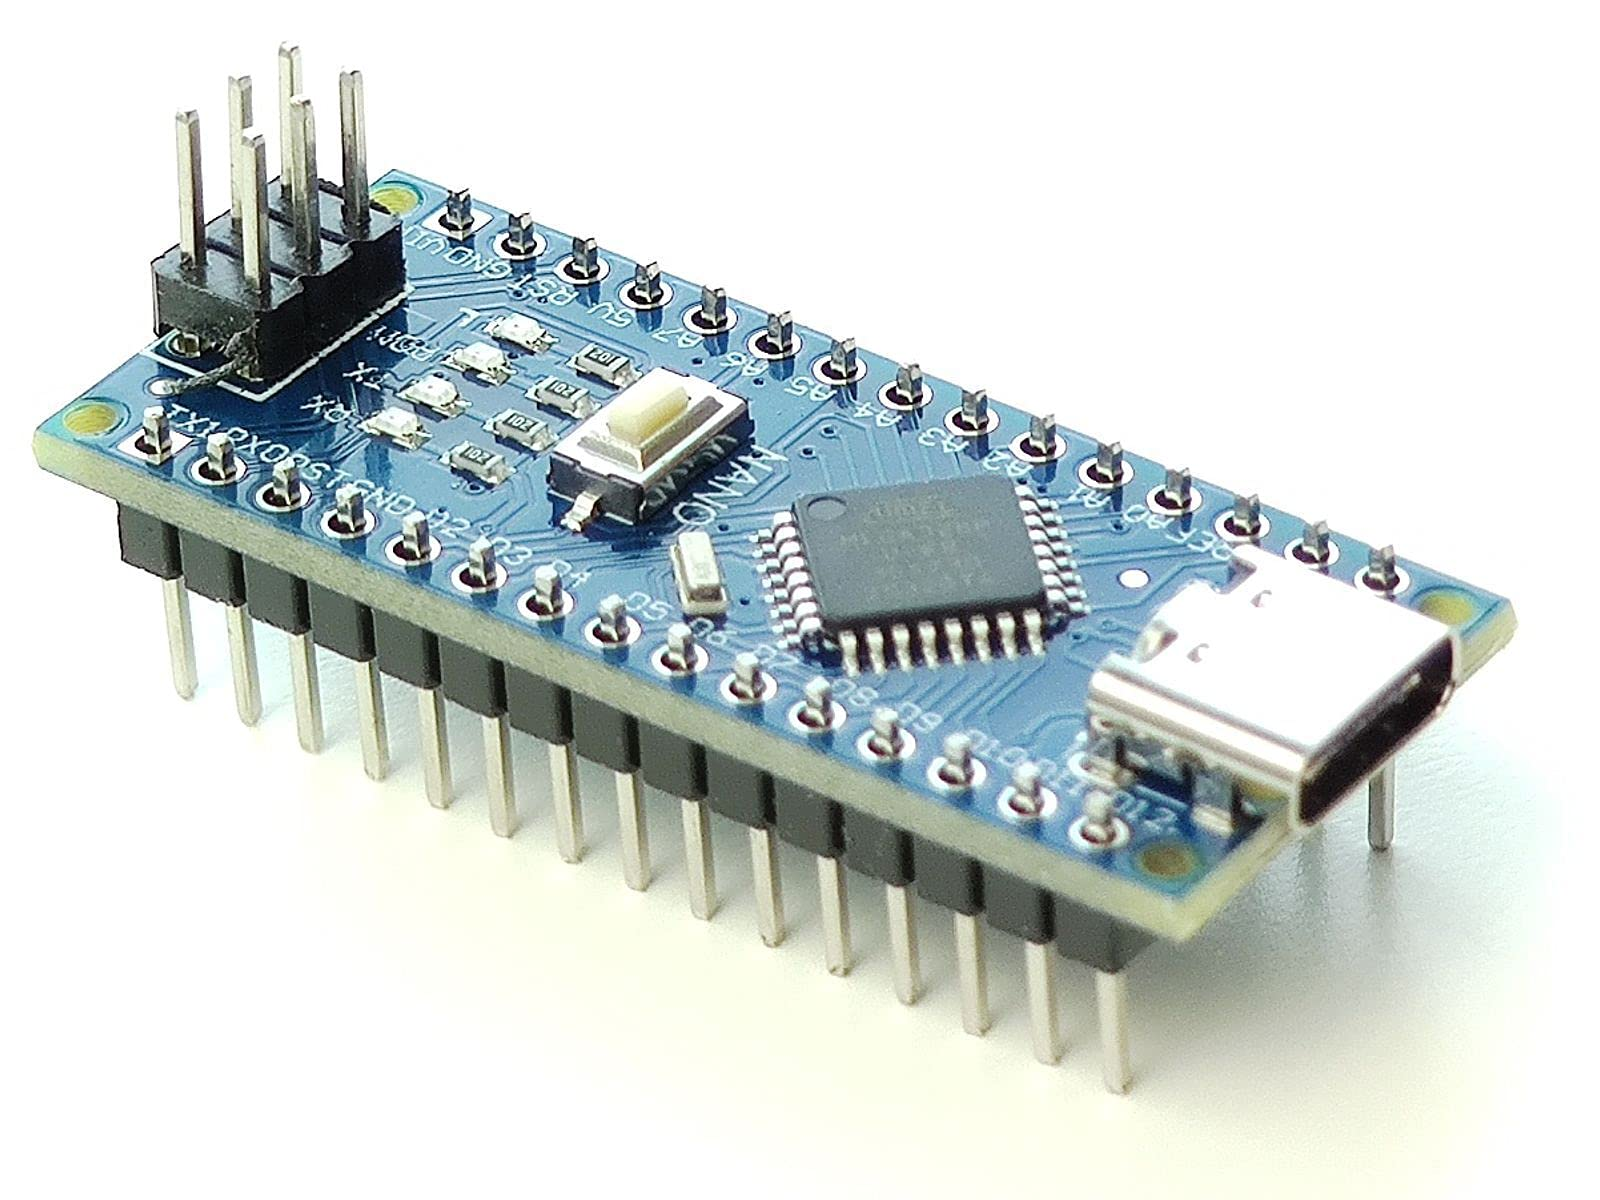
\includegraphics[width=0.5\textwidth]{graphicx/nano}
        \caption{The Arduino Nano with pin headers for GPIOs and USB-C connector to provide power and for uploading the code with a computer. \cite{nano}}
        \label{nano}
    \end{figure} 
    
    \subsection{Infrared Remote}

    
    \subsection{Infrared Receiver Module TSOP1736}
    \subsection{Servo Motor}
    \subsection{Reflective Sensor CNY70}

\section{Hardware design and development}
    \subsection{Block Diagram}
    \subsection{Schematic}
    \subsection{Hardware Setup}

\section{Software design and development}
    \subsection{Flowchart}
    \subsection{Functions}
            \subsubsection{Initialization Variable}
            \subsubsection{Setup Function}
            \subsubsection{Heartbeat Function}
            \subsubsection{Infrared Receiver Function}
            \subsubsection{First Button Function}
            \subsubsection{Second Button Function}
            \subsubsection{Third Button Function}
            \subsubsection{Software Source Code}
            
\section{Result}

\printbibliography

\end{document}
